%%%%%%%%%%%%%%%%%%%%%%%%%%%%%%%%%%%%%%%%%%%%%%%%%%%%%%%%
%%%%%%%%%%%%%%%%%%%%%%%%%%%%%%%%%%%%%%%%%%%%%%%%%%%%%%%%
\section[Analysis]{Search for a single produced \Tp~decaying into top and Higgs in the full hadronic final state}
\setcounter{tocdepth}{2}

\begin{frame}
\begin{center}
Search for a single produced \Tp~decaying into top and Higgs in the full hadronic final state at 8 TeV with 19.7 fb$^{-1}$
\end{center}
\end{frame}


\subsection{Introduction - Analysis Strategy}

\begin{frame}{Introduction - Analysis Strategy}
\vspace{-.5cm}
\begin{columns}

\begin{column}{.40\textwidth}
\begin{block}{}
\scriptsize{
As phenomenology study, but:
  \begin{itemize}
  \item Selection optimization $\to$ Better discrimination
  \item Refinement of \Tp~reconstruction
  \item $M(T')\in [600,1000]$ \GeVcc
  \item Real Data: 19.7 fb$^{-1}$
  \item \textbf{Data-driven background estimation}
  \end{itemize}
}
\tiny{
\textit{Signal simulated with MadGraph and Pythia 6}
}
\end{block}
\end{column}

\begin{column}{.60\textwidth}
  \begin{center}
    \includegraphics[width=0.65\textwidth]{Tprime_scheme.png}\\
  \end{center}
\vspace{-.2cm}
\resizebox{\textwidth}{!}{
\begin{tabular}{|c|c|c|}
\hline 
Samples & Cross-Section (pb) & Number of events\\
\hline
QCD\_Pt-120to170 & 16\(\times 10^4\) & 5.9M\\
QCD\_Pt-170to300 & 34\(\times 10^3\) & 5.8M\\
QCD\_Pt-300to470 & 18\(\times 10^2\) & 5.9M\\ 
QCD\_Pt-470to600 & 114 & 3.9M\\
QCD\_Pt-600to800 & 27 & 3.9M\\
QCD\_Pt-800to1000 & 3.5 & 3.9M\\
QCD\_HT-500To1000 & 84\(\times 10^2\) & 30M\\ 
QCD\_HT-1000ToInf & 2\(\times 10^2\) & 14M\\ 
TTJets\_MSDecays & 247.7 [NNLO] & 62M\\
TprimeJetToTH\_\textbf{M-700} & 0.144 & 99K \\
\hline
\end{tabular}
}
\end{column}
\end{columns}

\vspace{-.1cm}
\begin{block}{}\scriptsize
\textbf{MC samples only used for illustration}:
\begin{itemize}
\item Low statistics on QCD $\to$ Large statistical uncertainties 
\item Final background estimated from data
\end{itemize}
\end{block}

\end{frame}

\begin{frame}{Basic selection}
\vspace{-.2cm}

\begin{columns}
\begin{column}{.50\textwidth}
\begin{block}{}\scriptsize
\tiny{HLT: DiJet80\_DiJet60\_DiJet20 (\etal{3.0})}%
\\\scriptsize{
\resizebox{\textwidth}{!}{
\begin{tabular}{|c|c|c|c|}
\hline 
Selection & $N(j)\ge 6$ & $N(j)\ge 4$ & $N(j)\ge 2$ \\
\hline
\textbf{HLT} & \ptg{20} & \ptg{60} & \ptg{80} \\
\textbf{1st cut} & \ptg{30} & \ptg{70} & \ptg{90} \\
\hline
\end{tabular}
}\\
\textbf{2nd cut}: $N(j)[|\eta|<2.5]\ge 5$ and \\
\hspace{1.1cm} $N(extra\; j)[|\eta|<5]\ge 1$\\
\textbf{3rd cut}: $p_{T}(j_{1})>$150 GeV/c\\
\textbf{4th cut}: \HTg{550}\\
\textbf{5th cut}: $N^{CSVM}_{b}\ge 3$}%
\end{block}
%\vspace{-1.0cm}
%\begin{center}
%    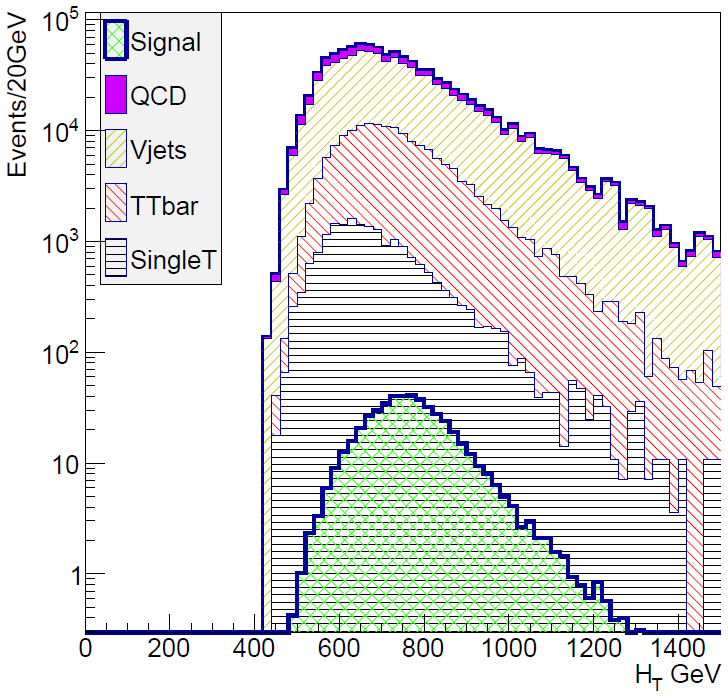
\includegraphics[width=0.7\textwidth]{../figs/Ana/HT.png}
%  \end{center}
\end{column}

\begin{column}{.50\textwidth}
\begin{figure}[!Hhtbp]
  \begin{center}
    \includegraphics[width=1.0\textwidth]{NCSVM.png}
  \end{center}
\end{figure}
\end{column}

\end{columns}

\end{frame}

\begin{frame}{\Tp~reconstruction with a $\chi^{2}$ sorting algorithm}
\vspace{-0.4cm}

\begin{center}
  \includegraphics[width=0.6\textwidth]{TprimeDecayChi2.png}
\end{center}

\vspace{-.5cm}
\tiny{
\begin{equation*}
\chi^{2}=\frac{(M_{H}-M_{bb})^{2}}{\sigma_{H}^{2}}+\frac{(M_{W}-M_{jj})^{2}}{\sigma_{W}^{2}}+\frac{(M_{t}-M_{bjj})^{2}}{\sigma_{t}^{2}}\; \text{to be minimized}
\end{equation*}
\vspace{-.2cm}
\begin{center}
$M_{H}=125$~\GeVcc, $M_{W}=84.06$~\GeVcc, $M_{t}=175.16$~\GeVcc\\
$\sigma_{H}=12.4$~\GeVcc, $\sigma_{W}=10.12$~\GeVcc, $\sigma_{t}=17.35$~\GeVcc
\end{center}
}%
\vspace{-.3cm}
\begin{center}
\includegraphics[width=0.54\textwidth]{Exclusive_Efficiency_V8.png}
\includegraphics[width=0.43\textwidth]{HundresdsMassChi2Tp.png}
\end{center}

\end{frame}


\begin{frame}{Selection based on reconstructed objects}
\vspace{-.2cm}
\scriptsize

\begin{columns}
\begin{column}{.50\textwidth}
\vspace{-.2cm}
\begin{block}{}
\tiny
\begin{itemize}
\item Optimization via a multidimensional scan of variables $\to$ adjusted to keep at least 10 signal events ($M(T')=700$~\GeVcc)
\item \textbf{Data/MC plot for illustration, final background estimation is data-derived}
\end{itemize}
\end{block}
\vspace{-.2cm}
\begin{block}{}\scriptsize
\textbf{1st criterion}: $\chi^{2}<8$, \tiny{${\epsilon(S)\sim 50\%,\; \epsilon(t\bar{t})\sim 30\%,\; \epsilon(QCD)\sim 3\%}$}\\
\scriptsize{
\textbf{2nd criterion}: $\Delta R(bb)<1.2$\\
\textbf{3rd criterion}: 105 $<M(H)<$ 145 \GeVcc\\
\textbf{4th criterion}: $(M(top^{2nd})+M(W^{2nd}))/M(H)>6.8$\\
\textbf{5th criterion}: $\Delta R (T' j^{6})>4.8$\\
\textbf{6th criterion}: Rel $H_{T}>0.67$}
\end{block}
\end{column}

\begin{column}{.50\textwidth}
\begin{figure}[!Hhtbp]
  \begin{center}
    \includegraphics[width=1.0\textwidth]{../figs/Ana/chi2Nm1.png}
  \end{center}
\end{figure}
\end{column}

\end{columns}

\end{frame}



\begin{frame}{Background shape estimation from data}
\vspace{-.2cm}

\begin{columns}
\begin{column}{.40\textwidth}
   \begin{block}{}\scriptsize
     \begin{itemize}
     \item Signal sample (SS): signal enriched \\$\to$ Standard selection
     \item Control sample (CS): background enriched $\to$ $n_{b}^{CSVL}>=3$ and veto $n_{b}^{CSVM}>=3$
     \item $M^{CS}(5j)$ to estimate $M^{SS}(5j)$
     \item Validation: 4 stages of selection (ABCD)
     %\textbf{Stage A}: Selection up to $\chi^{2}<8$, included.\\
     %\textbf{Stage B}: Selection up to $\Delta R(bb) <1.2$, included.\\
     %\textbf{Stage C}: Selection up to $\frac{M(top^{2nd}_{cand})+M(W^{2nd}_{cand})}{M(H_{cand})}>6.8$, included.\\
     %\textbf{Stage D}: Full selection.
     %\item Control vs signal sample for data~(A, B, C), \ttbar~MC~(A, B, C, D), QCD~MC~(A, B, C), MC samples sum~(A, B, C, D)%}%
     \item MC$^{CS}$ vs MC$^{SS}$, data$^{CS}$ vs data$^{SS}$
     \item Independence of WP for Control Sample: [0.244,0.679), [0.389,0.679), [0.534,0.679)
     \end{itemize}
    \end{block}

%\vspace{-.2cm}
%    \begin{block}{}\tiny
%      \textbf{Figure}: Schematic representation of signal and control sample. The big blue circle represents the ensemble of events with at least 3 CSVL b-tagged jets. The green circle represents the signal MC events while the circle filled with horizontal lines represents the signal sample (events with at least 3 CSVM b-tagged jets). The control sample then is the blue circle minus the horizontal line filled circle.
%    \end{block}
\end{column}

\begin{column}{.60\textwidth}
\begin{figure}[!Hhtbp]
  \begin{center}
    \includegraphics[width=1.0\textwidth]{../figs/Ana/SchematicControlSample.png}
  \end{center}
\end{figure}

\end{column}

\end{columns}

\end{frame}



\begin{frame}{Data-data}
\vspace{-.2cm}
\begin{figure}[!Hhtbp]
  \begin{center}
    \includegraphics[width=0.33\textwidth]{../figs/Ana/InclusiveVal_chi2_data.png}
    \includegraphics[width=0.33\textwidth]{../figs/Ana/InclusiveVal_DRWH_data.png}
    \includegraphics[width=0.33\textwidth]{../figs/Ana/InclusiveVal_M2HP_data.png}
    %\caption{Comparison of 5-jets invariant mass in signal sample and control sample. In the control sample, different b-tagging working points are studied. This comparison is done for data within 3 stages of selection: A [top left], B [top right] and C [bottom]. The 3 working points are given in different colors. Within statistical error, the 3 shapes for the control sample are in agreement at all stages with the signal sample, in gray. All histograms have been normalized to unity.}
    %\label{fig:StageWPData}
  \end{center}
\end{figure}

\vspace{-.2cm}
    \begin{block}{}\scriptsize
      \textbf{CS}: Three working points, three colors\\
      \textbf{SS}: Gray band\\
      Histograms normalized to unity $\to$ Shape comparison
    \end{block}

\end{frame}

\begin{frame}{\ttbar~MC-\ttbar~MC}
\vspace{-.2cm}
\begin{figure}[!Hhtbp]
  \begin{center}
    \includegraphics[width=0.42\textwidth]{../figs/Ana/InclusiveVal_chi2_ttbar.png}
    \includegraphics[width=0.42\textwidth]{../figs/Ana/InclusiveVal_DRWH_ttbar.png}
    %\includegraphics[width=0.25\textwidth]{../figs/Ana/InclusiveVal_M2HP_ttbar.png}
    %\includegraphics[width=0.25\textwidth]{../figs/Ana/InclusiveVal_RelHT_ttbar.png}
    %\caption{Comparison of 5-jets invariant mass in signal sample and control sample. In the control sample, different b-tagging working points are studied. This comparison is done for $t\bar{t}$ Monte Carlo samples within 4 stages of selection: A [top left], B [top right], C [bottom left] and D [bottom right]. The 3 working points are given in different colors. Within statistical error, the 3 shapes for the control sample are in agreement at all stages with the signal sample, in gray. \ttbar~MC as all the other Monte-Carlo samples are purely used for illustration. All histograms have been normalized to unity.}
    %\label{fig:StageWPttbar}
  \end{center}
\end{figure}

\vspace{-.2cm}
    \begin{block}{}\scriptsize
      \textbf{CS}: Three working points, three colors\\
      \textbf{SS}: Gray band\\
      Histograms normalized to unity $\to$ Shape comparison
    \end{block}

\end{frame}

\begin{frame}{\ttbar~MC-\ttbar~MC}
\vspace{-.2cm}
\begin{figure}[!Hhtbp]
  \begin{center}
    %\includegraphics[width=0.25\textwidth]{../figs/Ana/InclusiveVal_chi2_ttbar.png}
    %\includegraphics[width=0.25\textwidth]{../figs/Ana/InclusiveVal_DRWH_ttbar.png}
    \includegraphics[width=0.42\textwidth]{../figs/Ana/InclusiveVal_M2HP_ttbar.png}
    \includegraphics[width=0.42\textwidth]{../figs/Ana/InclusiveVal_RelHT_ttbar.png}
    %\caption{Comparison of 5-jets invariant mass in signal sample and control sample. In the control sample, different b-tagging working points are studied. This comparison is done for $t\bar{t}$ Monte Carlo samples within 4 stages of selection: A [top left], B [top right], C [bottom left] and D [bottom right]. The 3 working points are given in different colors. Within statistical error, the 3 shapes for the control sample are in agreement at all stages with the signal sample, in gray. \ttbar~MC as all the other Monte-Carlo samples are purely used for illustration. All histograms have been normalized to unity.}
    %\label{fig:StageWPttbar}
  \end{center}
\end{figure}

\vspace{-.2cm}
    \begin{block}{}\scriptsize
      \textbf{CS}: Three working points, three colors\\
      \textbf{SS}: Gray band\\
      Histograms normalized to unity $\to$ Shape comparison
    \end{block}

\end{frame}



\begin{frame}{Background normalization from data}
\vspace{-.2cm}

\begin{columns}
\begin{column}{.50\textwidth}
   \begin{block}{Method}\scriptsize
     \begin{itemize}
     \item Sideband from \tiny{${105~\text{GeV}/c^{2} <M(H_{cand})<145~\text{GeV}/c^{2}}$}%
     \item $N^{CS}_{in}$ and $N^{CS}_{out}\to R^{CS}=N^{CS}_{in}/N^{CS}_{out}$
     \item $R^{SS}=N^{SS}_{in}/N^{SS}_{out}$
     \end{itemize}
     \begin{equation*} 
      \text{if}\;\, R^{CS} = R^{SS}\Rightarrow N^{SS_{BKG}}_{in}=R^{CS}N^{SS}_{out}
     \end{equation*}
    \end{block}
\end{column}

\begin{column}{.50\textwidth}
\begin{block}{Validation}\scriptsize
\begin{itemize}
\item Hypothesis of $R^{CS} = R^{SS}$ (dominant backgrounds)
\item $N^{SS_{BKG}}_{in}=R^{CS}N^{SS}_{out}$ \MVAt~early selection stages
%\item $\chi^{2}$-test between the Higgs mass candidate in control and signal sample
\end{itemize}
\end{block}
\end{column}

\end{columns}

%\vspace{-.3cm}
\begin{center}
\resizebox{\textwidth}{!}{
\begin{tabular}{|c|c|c|c|c|}
\hline
 Cut & $R^{CS}$ & $R^{SS}$ & $N^{SS}_{in}$ & $N^{SS_{BKG}}_{in}$ \\
\hline
$\chi^{2}<8$ & $3.3\pm2.3\ex{-2}$ & $3.2\pm1.0\ex{-1}$ & $8100\pm90$ & $8400\pm220$ \\
$\Delta R(bb) <1.2$ & $2.7\pm3.7\ex{-2}$ & $2.7\pm1.3\ex{-1}$ & $2800\pm53$ & $2800\pm130$ \\
$\frac{M(top^{2nd}_{cand})+M(W^{2nd}_{cand})}{M(H_{cand})}>6.8$ & $2.4\pm4.4\ex{-2}$ & $2.4\pm1.7\ex{-1}$ & $1200\pm36$ & $1300\pm79$ \\
$ \Delta R (T' j^{6})>4.8$ & $2.5\pm1.6\ex{-1}$ & --- & --- & $98\pm22$ \\
$\frac{p_{T}(H_{cand})+p_{T}(top_{cand})}{H_{T}} > 0.67 $ & $2.7\pm3.1\ex{-1}$ & --- & --- & $53\pm18$ \\
\hline
\end{tabular}
}
\end{center}

\end{frame}


\begin{frame}{Signal extraction}
\vspace{-1.3cm}
\begin{columns}
\begin{column}{.50\textwidth}
   \begin{block}{}\scriptsize
     \begin{itemize}
     \item Gaussian fit for each mass point \\$\to$ $\mu, \; \sigma$
     \item To stabilize the statistical fluctuations of MC signal samples $\mu, \; \sigma$ fitted with a line
     \item Signal yield: Events in a 1-$\sigma$ window around the mean value of $M(5j)$ after full selection for each signal MC mass point
     \end{itemize}
    \end{block}

\end{column}

\begin{column}{.50\textwidth}
\begin{figure}[!Hhtbp]
  \begin{center}
    \includegraphics[width=0.9\textwidth]{Fitted_TpMass_V8.png}\\
    \includegraphics[width=0.9\textwidth]{Fitted_TpSigma_V8.png}
  \end{center}
\end{figure}
\end{column}

\end{columns}

%\vspace{-.2cm}
%\begin{center}
%\resizebox{0.58\textwidth}{!}{
\begin{textblock}{70}(2,70)
\resizebox{\textwidth}{!}{
\begin{tabular}{|c|c|c|c|c|}
\hline
\multicolumn{5}{|c|}{Results from linear fit} \\
Sample Name & Mass (GeV/$c^{2}$) & Width (GeV/$c^{2}$) & Yield & Error on yield (\%)\\
\hline
$Tj\rightarrow tHj$ 600 GeV/$c^{2}$ & 601 & 34 & $4.4\pm0.4$ & 7.9\% \\
$Tj\rightarrow tHj$ 650 GeV/$c^{2}$ & 647 & 37 & $6.6\pm0.4$ & 5.7\% \\
$Tj\rightarrow tHj$ 700 GeV/$c^{2}$ & 693 & 39 & $7.8\pm0.4$ & 4.7\% \\
$Tj\rightarrow tHj$ 750 GeV/$c^{2}$ & 740 & 42 & $7.2\pm0.3$ & 4.5\% \\
$Tj\rightarrow tHj$ 800 GeV/$c^{2}$ & 786 & 44 & $6.1\pm0.3$ & 4.6\% \\
$Tj\rightarrow tHj$ 850 GeV/$c^{2}$ & 833 & 47 & $5.7\pm0.2$ & 4.3\% \\
$Tj\rightarrow tHj$ 900 GeV/$c^{2}$ & 879 & 50 & $4.8\pm0.2$ & 4.3\% \\
$Tj\rightarrow tHj$ 950 GeV/$c^{2}$ & 925 & 52 & $3.8\pm0.2$ & 4.6\% \\
$Tj\rightarrow tHj$ 1000 GeV/$c^{2}$ & 972 & 55 & $2.3\pm0.1$ & 5.4\% \\
\hline
\end{tabular}
}
\end{textblock}
%\end{center}

\end{frame}



\begin{frame}{Systematics uncertainties}
\vspace{-.2cm}

\begin{block}{}\scriptsize
Variation of signal and background yields when uncertainties sources are varied within their errors:
  \begin{itemize}
  \item Signal $\to$ MC corrections varied between errors: JES, Pileup, B-tagging, PDF, trigger
  %\item If the variation of the yield for a given uncertainty source is contained in the statistical error of the yield, the statistical error is taken as the value of the uncertainty due to the uncertainty source
  \item Background: Validation of estimation methods
  \item Quoted as $(Y'-Y)/Y$ in \%
  \end{itemize}
\end{block}

\begin{center}
\resizebox{0.85\textwidth}{!}{
\begin{tabular}{|c|c|c|}
\hline
Systematics Name & Signal $M(T')=700$~\GeVcc & Background \\
\hline
%Theory & 5\% & --\\                                                                                                                                                                                       
PDF & 4.7\% & --\\
Luminosity & 2.6\% & --\\
Trigger & 4.7\% & --\\
B-tag & +6.2\% / -5.9\% & --\\
JEC & +4.7\% / - 6.2\% & --\\
Pileup & 4.7\% & --\\
Background Shape determination & -- & 20\%\\
Background Normalization & -- & 34\%\\
\hline
\end{tabular}
}
\end{center}

\end{frame}

\begin{frame}{Statistical interpretation}
\vspace{-.6cm}
\begin{columns}
\begin{column}{.50\textwidth}\tiny
\begin{block}{\scriptsize{Cut-and-count experiment}}\tiny
Test compatibility of data with hypotheses - frequentist approach:
\begin{itemize}
\item Model: ${\lambda(\beta,\theta)=\beta S(\theta)+B(\theta)}$
\item Poisson-like distributions
\item Likelihood: $L(\beta,\theta)=\frac{\lambda(\beta,\theta)^{n}}{n!}e^{-\lambda(\beta,\theta)}$
\item Test statistic: $q=-2ln(L_{s+b}/L_{b})$
\item Probability distribution function per hypothesis: $f(q|s+b)$, $f(q|b)$ $\to$ Integral to the right is the p-value $\alpha$
\item Upper limit on $\beta$ at a confidence level $CL=1-\alpha$ 
\item $CL_{s}=CL_{s+b}/CL_{b}$, with $CL_{s}=0.05$ is exclusion~\MVAt~95\% CL 
\end{itemize}
\end{block}
\end{column}

\begin{column}{.50\textwidth}\tiny
\begin{figure}[!Hhtbp]
  \begin{center}
    \includegraphics[width=1.0\textwidth]{../figs/Ana/stats1.png}
    %\caption{The distribution of the test statistics $q=-2ln(L_{s+b}/L_{b})$ under the hypothesis of $\beta=0$ (null signal hypothesis) and $\beta=1$ (positive signal hypothesis)~\cite{stats1}. $q_{obs}$ is the observed value of $q$ in data, $p_{s+b}$ and $p_{b}$ the probabilities the observation come from the positive signal and null signal hypotheses, correspondingly.}
    %\label{fig:stats1}
  \end{center}
\end{figure}
\end{column}

\end{columns}

\end{frame}

\begin{frame}{Results}
\vspace{-.6cm}

\begin{columns}
\begin{column}{.50\textwidth}\tiny
\begin{figure}[!Hhtbp]
  \begin{center}
    \includegraphics[width=0.9\textwidth]{../figs/Ana/Final_Plot_NoSubs.png}
    %\caption{$M(5j)$ after full selection for data and the estimated background and signal mass points at 650 \GeVcc~and 850 \GeVcc.}
    %\label{fig:FinalPlot2}
  \end{center}
\end{figure}
\vspace{-.2cm}
\begin{block}{}\tiny
$M(5j)$ after full selection for data and the estimated background and signal mass points at 650 \GeVcc~and 850 \GeVcc.
\end{block}
\end{column}

\begin{column}{.50\textwidth}\tiny
%\begin{figure}[!Hhtbp]
  \begin{center}
    \includegraphics[width=1.0\textwidth]{Limits_from_CLs_V8_LinearFitWidths_1sigma_Revision.png}
  \end{center}
%\end{figure}
\vspace{-.2cm}
\begin{block}{}\tiny
Expected and observed limits in terms of \Tp~production cross section as a function of $M(5j)$. Observed limits: 850~\GeVcc and 813-862 \GeVcc~from linear interpolation excluded at 95\% CL. \textcolor{red}{Theory prediction (non-standard doublet, maximized couplings to light quarks)}
\end{block}
\end{column}

\end{columns}

\end{frame}



%%%%%%%%%%%%%%%%%%%%%%%%%%%%%%%%%%%%%%%%%%%%%%%%%%%%%%%%%%%%%%%%%%%%%%%%%%%%%%%%%%%%%%%%%%%%%%%%%%%%%%%%%%%%%%%%%%%%

\iffalse
\begin{frame}{Introduction - Analysis Strategy}
\vspace{-.2cm}
\begin{columns}

\begin{column}{.50\textwidth}
\begin{block}{}
\begin{itemize}\scriptsize
\item Single produced \Tp~with an associated jet
\item Full hadronic final state: \\ $T'\to t H \to b W^{+} \bar{b} b \to b \bar{b} j j b$
\item Reconstruction of \Tp~mass: $M(5j)$
\item Main challenges:
  \begin{itemize}\scriptsize
  \item Huge backgrounds $\rightarrow$ Mainly QCD and \ttbar
  \item \Tp~reconstruction with high jet multiplicity
  \end{itemize}
\item Fundamental tools for background discrimination:
  \begin{itemize}\scriptsize
  \item B-tagged jets multiplicity
  \item \Tp~reconstruction procedure
  \end{itemize}
\end{itemize}
\end{block}
\end{column}

\begin{column}{.50\textwidth}
\begin{center}
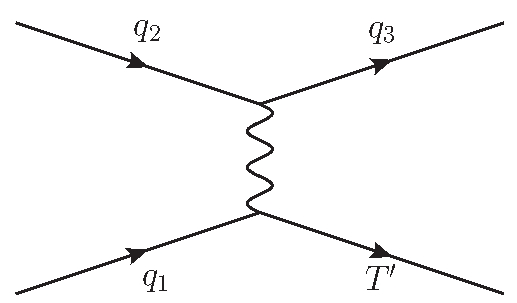
\includegraphics[width=0.9\textwidth]{../figs/Tchannel_T_single.jpg}\\
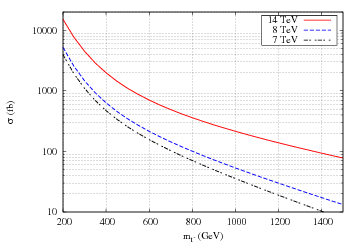
\includegraphics[width=1.0\textwidth]{../figs/pheno_prod_single_tp.png}
\end{center}
\end{column}
\end{columns}

\end{frame}

\begin{frame}{Datasets}
\vspace{-.2cm}

%\begin{table*}[htbH]
\begin{center}
\resizebox{\textwidth}{!}{
\begin{tabular}{|c|c|}
\hline 
Dataset name & Int. Luminosity ($\text{pb}^{-1}$) \\
\hline
/MultiJet/Run2012A-22Jan2013-v1/AOD & 889.4 \\
/MultiJet1Parked/Run2012B-05Nov2012-v2/AOD & 4429.0 \\
/MultiJet1Parked/Run2012C-part1-05Nov2012-v2/AOD & 494.6 \\
/MultiJet1Parked/Run2012C-part2-05Nov2012-v2/AOD & 6654.0 \\
/MultiJet1Parked/Run2012D-part1-10Dec2012-v1/AOD & 5955.1 \\
/MultiJet1Parked/Run2012D-part2-17Jan2013-v1/AOD & 734.0 \\
/MultiJet1Parked/Run2012D-part2-PixelRecover-17Jan2013-v1 & 538.4 \\
\hline
\multicolumn{1}{|r|}{\textit{Total}} & 19694.5 \\
\hline
\end{tabular}
}
%\caption{List of Multijet Primary Dataset used in the analysis and the corresponding integrated luminosity calculated using the golden JSON (Java Script Object Notation) file. The golden JSON file contains the information about the luminosity sections considered as good for all runs. A good luminosity section is defined as a luminosity section where the detector was fully functioning, this is all subsystems were taking data and without problems.  \label{tab:datasets}}
\end{center}
%\end{table*}

%\begin{table*}[htbH]
\begin{center}
\resizebox{\textwidth}{!}{
\begin{tabular}{|c|c|c|}
\hline 
Samples & Cross-Section (pb) & Number of events\\
\hline
QCD\_Pt-120to170\_TuneZ2star\_8TeV\_pythia6 & 16\(\times 10^4\) & 5.9M\\
QCD\_Pt-170to300\_TuneZ2star\_8TeV\_pythia6 & 34\(\times 10^3\) & 5.8M\\
QCD\_Pt-300to470\_TuneZ2star\_8TeV\_pythia6 & 18\(\times 10^2\) & 5.9M\\ 
QCD\_Pt-470to600\_TuneZ2star\_8TeV\_pythia6 & 114 & 3.9M\\
QCD\_Pt-600to800\_TuneZ2star\_8TeV\_pythia6 & 27 & 3.9M\\
QCD\_Pt-800to1000\_TuneZ2star\_8TeV\_pythia6 & 3.5 & 3.9M\\
QCD\_HT-500To1000\_TuneZ2star\_8TeV-madgraph-pythia6 & 84\(\times 10^2\) & 30M\\ 
QCD\_HT-1000ToInf\_TuneZ2star\_8TeV-madgraph-pythia6 & 2\(\times 10^2\) & 14M\\ 
TTJets\_MSDecays\_central\_TuneZ2star\_8TeV-madgraph-tauola & 247.7 [NNLO] & 62M\\
TprimeJetToTH\_\textbf{M-700}\_TuneZ2star\_8TeV-madgraph\_tauola & 143.7 & 99K \\
\hline
\end{tabular}
}
%\caption{List of Monte-Carlo background samples used in the analysis, their corresponding cross-section and their number of events.\label{tab:MCbkg}}
\end{center}
%\end{table*}

\tiny{Signal samples were done with $T'\to tH$ with $H\to\tau^{+}\tau^{-}$ (6\%) and $H\to b\bar{b}$ (94\%). Correction with weight of 0.61 to obtain correct $Br(H\to b\bar{b})=0.57$. }

\end{frame}

\begin{frame}{Event selection}
\vspace{-.2cm}

\begin{columns}

\begin{column}{.55\textwidth}
\begin{block}{Event processing}
\begin{itemize}\scriptsize
  \item Data processed using ``golden'' JSON file: Consider only validated lumi sections
  \item PAT processing
    \begin{itemize}\tiny
    \item Jets reconstructed with PF algorithm and CHS
    \item Jets: \ptg{20} and $|\eta|<5$
    \item At least one good primary vertex: $\text{n.d.o.f.} \ge 4,\; |z|<24 \;\text{cm},\; |\rho|< 2 \;\text{cm}$
    \item Global tag: Calibration and alignment info for data, MC corrected to get close to data conditions
    \end{itemize}
  \item Pile-up corrections: Simulated PU in MC was corrected to observed PU in Data
\end{itemize}
\end{block}
\end{column}

\begin{column}{.45\textwidth}
\vspace{-.9cm}
\begin{figure}[!Hhtbp]
  \begin{center}
    \includegraphics[width=1.0\textwidth]{../figs/Ana/Nvtcs.png}
  \end{center}
\end{figure}
\vspace{-.75cm}
\begin{block}{}
\tiny Number of vertices distribution for data and MC samples. The comparison has been performed after basic selection except number of b-tagged jets (the basic selection is described in the next slides). The gray band correspond to the statistical error of MC samples sum. Normalization of MC samples was done to the 19.7~fb$^{-1}$.
\end{block}
\end{column}

\end{columns}
\end{frame}

\begin{frame}{Basic selection}
\vspace{-.2cm}

\begin{block}{}
  \begin{itemize}\scriptsize
  \item Trigger L1: at least 4 central jets (\etal{3}) with \ptg{32}~or \ptg{36}~or \ptg{40} \\
                    or at least 2 central jets with \ptg{52}~or \ptg{56}~or \ptg{64} \\
                    or events with \HTg{125}~or \HTg{150}~or \HTg{175}
  \item HLT: 6 central jets with a \ptg{20}, 4 with a \ptg{60} and 2 with a \ptg{80}
  \item \textbf{First offline cut}: 2 jets with \ptg{90}, 2 jets with \ptg{70} and 2 jets with \ptg{30}
  \end{itemize}
\end{block}

\begin{columns}
\begin{column}{.50\textwidth}
\vspace{-.2cm}
\begin{block}{}
  \scriptsize \textbf{Second cut}: At least 5 jets with \ptg{30} and \etal{2.5} and at least one additional jet with \ptg{30} and \etal{5} were required
\end{block}

\vspace{-.2cm}
\begin{block}{}
\scriptsize \textbf{Figure}: Distribution of pseudorapidity of the accompanying jet produced with the \Tp. The distribution is taken from the signal MC sample with M=700 \GeVcc~and it is normalized to unity.
\end{block}
\end{column}

\begin{column}{.50\textwidth}
\vspace{-.2cm}
\begin{figure}[!Hhtbp]
  \begin{center}
    \includegraphics[width=1.0\textwidth]{../figs/Ana/SixthJetMCTruth.png}
    %\caption{Distribution of pseudorapidity of the accompanying jet produced with the \Tp. The distribution is taken from the signal MC sample with M=700 \GeVcc~and it is normalized to unity.}
    %\label{fig:SixthJetTp}
  \end{center}
\end{figure}
\end{column}
\end{columns}

\end{frame}

\begin{frame}{}
\vspace{-.2cm}

\begin{columns}
\begin{column}{.50\textwidth}
\begin{block}{}
\scriptsize \textbf{3rd cut}: the leading jet was required to have a \ptg{150}
\end{block}
\vspace{-.2cm}
\begin{block}{}
\scriptsize \textbf{4th cut}: \HTg{550} was required
\end{block}
\vspace{-.2cm}
\begin{block}{}
\scriptsize \textbf{Figure}: Distribution of the $H_{T}$ variable for data and the sum of the MC samples normalized to luminosity. The signal sample (M=700 \GeVcc) is over-imposed on top of the stack of the MC samples. The gray band represents the statistical uncertainties from the sum of the MC background. Reasonable agreement is observed, with the multijet process as the dominant process at this stage. Normalization of samples was done to luminosity.
\end{block}
\end{column}

\begin{column}{.50\textwidth}
\begin{figure}[!Hhtbp]
  \begin{center}
    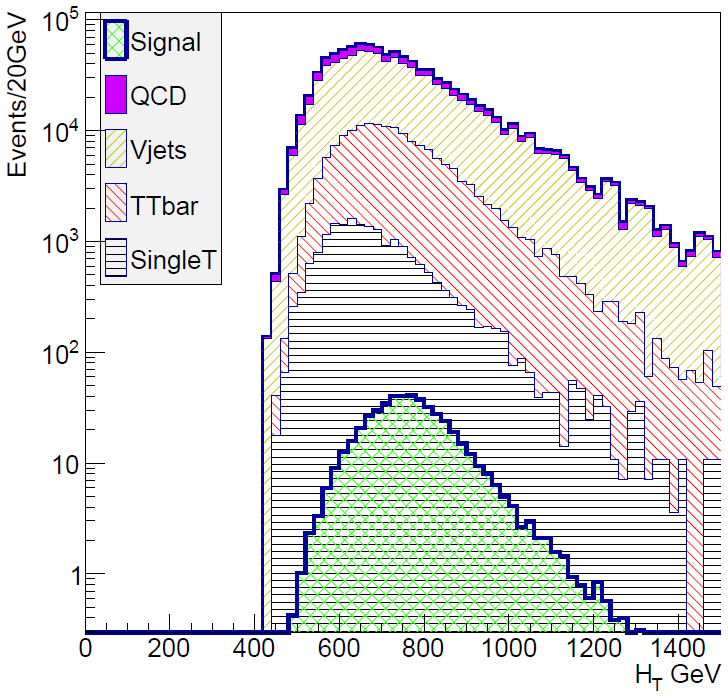
\includegraphics[width=1.0\textwidth]{../figs/Ana/HT.png}
    %\caption{Distribution of the $H_{T}$ variable for data and the sum of the MC samples normalized to luminosity. The signal sample (M=700 \GeVcc) is over-imposed on top of the stack of the MC samples. The gray band represents the statistical uncertainties from the sum of the MC background. Reasonable agreement is observed, with the multijet process as the dominant process at this stage. Normalization of samples was done to luminosity.}
    %\label{fig:HT}
  \end{center}
\end{figure}
\end{column}

\end{columns}
\end{frame}

\begin{frame}{}
\vspace{-.2cm}

\begin{columns}
\begin{column}{.50\textwidth}
\begin{block}{}
\scriptsize \textbf{B-tagging}: CSV (Constrained Secondary Vertex) algorithm $\to$ Multivariate technique that give a discriminator indicating how likely a jet is coming from a b-quark
\textbf{Working points}: Loose, Medium and Tight\\\tiny{CSVL$\to$0.244 \\$\epsilon^{CSVL}_{b}=85$\%, $\epsilon^{CSVL}_{c}=45$\%, $\epsilon^{CSVL}_{l}=10$\% \\CSVM$\to$0.679\\ $\epsilon^{CSVM}_{b}=$70\%, $\epsilon^{CSVM}_{c}=$20\%, $\epsilon^{CSVM}_{l}=$1\% \\CSVT$\to$0.898\\ $\epsilon^{CSVT}_{b}=50$\%, $\epsilon^{CSVT}_{c}=7$\%, $\epsilon^{CSVT}_{l}=0.2$\%}
\end{block}
\vspace{-.2cm}
\begin{block}{}
\scriptsize \textbf{5th cut}: at least 3 CSVM b-tagged jets. Only jets with $|\eta|<=2.4$ considered for b-tagging.
\end{block}
\vspace{-.2cm}
\begin{block}{}
\scriptsize \textbf{Figure}: B-tagged CSVM jet multiplicity for data and MC samples before requiring at least 3 CSVM b-tagged jets. The sum of MC samples is normalized to the integrated luminosity.
\end{block}
\end{column}

\begin{column}{.50\textwidth}
\begin{figure}[!Hhtbp]
  \begin{center}
    \includegraphics[width=1.0\textwidth]{../figs/Ana/NCSVM.png}
    %\caption{B-tagged CSVM jet multiplicity for data and MC samples before requiring at least 3 CSVM b-tagged jets. The sum of MC samples is normalized to the integrated luminosity.}
    %\label{fig:Nb}
  \end{center}
\end{figure}
\end{column}

\end{columns}
\end{frame}



%\begin{frame}{Corrections to MC for b-tagging}
%\vspace{-.2cm}
%
%\begin{columns}
%\begin{column}{.50\textwidth}
%\begin{block}{}
%\scriptsize Scale factors derived from data/MC comparisons $\to$ $SF^{flavor}_{\eta}(p_{T})$\\
%As mean values: $SF^{b\; or\; c}\sim 0.94$ and $SF^{light}\sim 1.06$
%\end{block}
%\vspace{-.2cm}
%\begin{block}{}
%\scriptsize In order to apply the SF's a weight per event is calculated\\
%$w=\frac{P(\text{DATA})}{P(\text{MC})}$ with \\ \tiny{
%$P(\text{MC}) = \prod_{i=\text{tagged}} \varepsilon_i \prod_{j=\text{not tagged}} (1-\varepsilon_j)$\\
%$P(\text{DATA}) = \prod_{i=\text{tagged}} \text{SF}_i \varepsilon_i \prod_{j=\text{not tagged}} (1-\text{SF}_j \varepsilon_j)$ \\
%}
%\end{block}
%\vspace{-.2cm}
%\begin{block}{}
%\tiny B-tagging efficiencies defined as\\
%$\varepsilon_f(i,j) = \frac{N_f^\text{b-tagged}(i,j)}{N_f^\text{Total}(i,j)}$ where \\
%where $ N_f^\text{Total}(i,j) $ and $ N_f^\text{b-tagged}(i,j) $ are the total number and the number of b-tagged jets, respectively, of flavor $ f $ in the $ (p_\text{T},\eta) $ bin $ (i,j) $ for a given MC sample.
%\end{block}
%\vspace{-.2cm}
%\begin{block}{}
%\scriptsize \textbf{Figure}: Distribution of the weights from b-tagging scale factors for all MC samples.
%\end{block}
%\end{column}
%
%\begin{column}{.50\textwidth}
%\begin{figure}[!Hhtbp]
%  \begin{center}
%    \includegraphics[width=1.0\textwidth]{../figs/Ana/SF_weight.png}
    %\caption{Distribution of the weights from b-tagging scale factors for all MC samples.}
    %\label{fig:SFweight}
%  \end{center}
%\end{figure}
%\end{column}

%\end{columns}
%\end{frame}

\begin{frame}{\Tp~reconstruction with a $\chi^{2}$ sorting algorithm}
\vspace{-.2cm}
\scriptsize

\begin{itemize}
\item $\chi^{2}$ sorting algorithm used to identify the \Tp~decay products and to reconstruct the Higgs and top candidates
\item $\chi^{2}$ variable defined for each jets combination in an event
\item The combination that minimizes this variable gives the best fit of the objects under reconstruction
\end{itemize}

\begin{equation*}
\chi^{2}=\frac{(M_{H}-M_{bb})^{2}}{\sigma_{H}^{2}}+\frac{(M_{W}-M_{jj})^{2}}{\sigma_{W}^{2}}+\frac{(M_{t}-M_{bjj})^{2}}{\sigma_{t}^{2}}
%\label{eq:chi2def}
\end{equation*}

\begin{itemize}
\item $M_{H}=125$~\GeVcc, $M_{W}=84.06$~\GeVcc, $M_{t}=175.16$~\GeVcc, $\sigma_{H}=12.4$~\GeVcc, and $\sigma_{W}=10.12$~\GeVcc~and $\sigma_{t}=17.35$~\GeVcc. From similar MC studies.
\item For the Higgs reconstruction only CSVM b-tagged jets were considered
\item For the \W~reconstruction all jets with a \ptg{30} were considered
\item For the top reconstruction one b-tagged jet and the pair of jets used for the \W~were utilized
\end{itemize}

\end{frame}

\begin{frame}{}
\vspace{-.2cm}

\begin{columns}
\begin{column}{.50\textwidth}

\begin{figure}[!Hhtbp]
  \begin{center}
    \includegraphics[width=1.0\textwidth]{../figs/Ana/Exclusive_Efficiency_V8.png}
    %\includegraphics[width=0.46\textwidth]{figs/Ana/Inclusive_Efficiency_V8.png}
    %\caption{Reconstruction efficiency by the $\chi^{2}$ algorithm of the Higgs boson, \W~boson, top quark and \Tp, as the ratio of the number of events where the particle was correctly reconstructed to the number of events where jets could be matched to partons [left] and to the total number of events [right]}
    %\label{fig:RecEff}
  \end{center}
\end{figure}

\vspace{-.2cm}
\begin{block}{}
\scriptsize \textbf{Figure}: Reconstruction efficiency by the $\chi^{2}$ algorithm of the Higgs boson, \W~boson, top quark and \Tp, as the ratio of the number of events where the particle was correctly reconstructed to the number of events where jets could be matched to partons.
\end{block}
\end{column}

\begin{column}{.50\textwidth}

\begin{figure}[!Hhtbp]
  \begin{center}
    \includegraphics[width=1.0\textwidth]{../figs/Ana/HundresdsMassChi2Tp.png}
    %\includegraphics[width=0.45\textwidth]{figs/Ana/FiftiesMassChi2Tp.png}
    %\caption{Reconstructed \Tp~mass for all mass points from the $\chi^{2}$ sorting algorithm after basic selection. Each mass point is normalized to luminosity and its corresponding cross section. A gaussian fit of these distributions will be presented afterward in section~\ref{sec:finalsel}, accompanied with a discussion about the resolution on the reconstruction of the \Tp.}
    %\label{fig:RecT}
  \end{center}
\end{figure}

\vspace{-.2cm}
\begin{block}{}
\scriptsize \textbf{Figure}: Reconstructed \Tp~mass for some mass points from the $\chi^{2}$ sorting algorithm after basic selection. Each mass point is normalized to luminosity and its corresponding cross section.
\end{block}
\end{column}

\end{columns}
\end{frame}

\begin{frame}{Selection based on reconstructed objects}
\vspace{-.2cm}
\scriptsize

\begin{columns}
\begin{column}{.50\textwidth}
\vspace{-.2cm}
\begin{block}{}
\tiny
\begin{itemize}
\item Selection optimized via a multidimensional scan of variables 
\item Signal discrimination evaluated by $S/B$, using as signal the $M=700$\GeVcc~mass point, and as background the \ttbar~and QCD\_HT-500To1000
\item Selection has been adjusted to keep at least 10 signal events, for the 700~\GeVcc~mass point, after the full selection
\item \textbf{Data/MC plots are shown for illustration, but final background estimation is derived from data}
\end{itemize}
\end{block}
\vspace{-.2cm}
\begin{block}{}
\scriptsize \textbf{1st criterion}: $\chi^{2}<8$
\end{block}
\vspace{-.2cm}
\begin{block}{}
\scriptsize \textbf{Figure}: Distribution of the $\chi^{2}$ variable for data and MC samples. The signal sample used has a \Tp~mass of 700 \GeVcc. Backgrounds present higher values than the signal. The sum of MC is normalized to the integrated luminosity.
\end{block}
\end{column}

\begin{column}{.50\textwidth}
\begin{figure}[!Hhtbp]
  \begin{center}
    \includegraphics[width=1.0\textwidth]{../figs/Ana/chi2Nm1.png}
    %\caption{Distribution of the $\chi^{2}$ variable for data and MC samples. The signal sample used has a \Tp~mass of 700 \GeVcc. Backgrounds present higher values than the signal. The sum of MC is normalized to the integrated luminosity. }
    %\label{fig:chi2}
  \end{center}
\end{figure}
\end{column}

\end{columns}

\end{frame}

\begin{frame}{}
\vspace{-.2cm}
    \begin{block}{}\scriptsize
      \textbf{2nd criterion}: $\Delta R(bb)<1.2$\\
      \textbf{3rd criterion}: Higgs candidate mass between 105 and 145 \GeVcc
    \end{block}

\vspace{-.5cm}
\begin{columns}
\begin{column}{.50\textwidth}
\begin{figure}[!Hhtbp]
  \begin{center}
    \includegraphics[width=0.9\textwidth]{../figs/Ana/DRbbNm1.png}
  \end{center}
\end{figure}

\vspace{-.7cm}
    \begin{block}{}\tiny
      $\Delta R$ of the 2 b-tagged jets used to reconstruct the Higgs candidate after $\chi^{2}$ cut.
    \end{block}
\end{column}

\begin{column}{.50\textwidth}
\begin{figure}[!Hhtbp]
  \begin{center}
    \includegraphics[width=0.9\textwidth]{../figs/Ana/HMNm1.png}
  \end{center}
\end{figure}

\vspace{-.7cm}
    \begin{block}{}\tiny
      Distribution for $M(H_{cand})$ for data and the sum of Monte Carlo samples. All others selection criteria are applied up to this one.
    \end{block}
\end{column}

\end{columns}

\end{frame}


\begin{frame}{}
\vspace{-.2cm}
    \begin{block}{}\scriptsize
      \textbf{4th criterion}: $(M(top^{2nd})+M(W^{2nd}))/M(H)>6.8$\\
      \textbf{5th criterion}: $\Delta R (T' j^{6})>4.8$\\
      \textbf{6th criterion}: $H_{T}>0.67$
    \end{block}

\vspace{-.5cm}
\begin{columns}
\begin{column}{.50\textwidth}
\begin{figure}[!Hhtbp]
  \begin{center}
    \includegraphics[width=0.8\textwidth]{../figs/Ana/M2HPNm1.png}
  \end{center}
\end{figure}

\vspace{-.7cm}
    \begin{block}{}\tiny
      Distribution of $(M(top^{2nd})+M(W^{2nd}))/M(H)$ for data and the sum of the Monte Carlo samples. Selection criteria are applied up to Higgs mass cut. The low statistics in the multijet (QCD) MC sample is visible at this stage.
    \end{block}
\end{column}

\begin{column}{.50\textwidth}
\begin{figure}[!Hhtbp]
  \begin{center}
    \includegraphics[width=0.8\textwidth]{../figs/Ana/DRTp6JNm1.png}
  \end{center}
\end{figure}

\vspace{-.7cm}
    \begin{block}{}\tiny
      Distributions for $\Delta R (T' j^{6})$  for data and the sum of Monte Carlo samples. All others criteria are applied up to this one. The low statistics in the multijet (QCD) MC sample is visible at this stage.
    \end{block}
\end{column}

\end{columns}

\end{frame}

%\begin{frame}{Selection optimization}
%\vspace{-.2cm}
%
%\begin{table}[htbH]
%\begin{center}
%\resizebox{\textwidth}{!}{
%\begin{tabular}{|c|c|c|}
%\hline 
%Cut & $S/B$ & $S/\sqrt{S+B}$ \\
%\hline
%$\chi^{2}<8$ & $3.4\ex{-2} \pm 2.85\ex{-3}$  & $ 0.96 \pm 0.05$  \\
%$\Delta R(bb)<1.2$ & $4.76\ex{-2} \pm 4.52\ex{-3}$ & $1.10 \pm 0.07$  \\
%%$1.6<\Delta R (W_{cand} H_{cand})<4.0$ & $4.82\ex{-2} \pm 4.59\ex{-3}$  & $1.10 \pm 0.07$  \\
%$105$ \GeVcc~$< M(H_{cand}) < 145$ \GeVcc~& $6.37\ex{-2} \pm 6.74\ex{-3}$  & $1.22 \pm 0.08$  \\
%$(M(top^{2nd})+M(W^{2nd}))/M(H_{cand})>6.8$ & $0.15 \pm 0.03$  & $1.45 \pm 0.16$  \\
%$\Delta R (T j^{6})>4.8$ & $0.42 \pm 0.19$  & $1.67 \pm 0.32$  \\
%Relative $H_{T}>0.67$ & $1.16 \pm 0.17$  & $2.13 \pm 0.17$  \\
%\hline
%\end{tabular}
%\caption{$S/B$ and $S/\sqrt{S+B}$ from MC samples for each step of the selection after reconstruction of resonances with the $\chi^{2}$ sorting algorithm. Only $M=700$ \GeVcc~signal, \ttbar~and QCD\_HT-500To1000 MC samples were used. \label{tab:Estimators}}
%}
%\end{center}
%\end{table}
%
%\vspace{-.2cm}
%    \begin{block}{}\scriptsize
%      $S/B$ and $S/\sqrt{S+B}$ from MC samples for each step of the selection after reconstruction of resonances with the $\chi^{2}$ sorting algorithm. Only $M=700$ \GeVcc~signal, \ttbar~and QCD\_HT-500To1000 MC samples were used.
%    \end{block}
%
%\end{frame}

\begin{frame}{Trigger efficiency}
\vspace{-.2cm}

\begin{columns}
\begin{column}{.50\textwidth}
   \begin{block}{}\scriptsize
     \begin{itemize}
     \item Prescaled trigger requiring \HTg{400} as reference.
     \item The \pt~of the 6th leading jet has been used to parametrize the trigger efficiency.
     \item Efficiency = number of events passing analysis and reference triggers / number of events passing only HLT\_HT400
     \end{itemize}
    \end{block}

\vspace{-.2cm}
    \begin{block}{}\tiny
      \textbf{Figure}: Efficiency in data and the MC signal samples for events passing trigger bit HLT\_Dijet80\_Dijet60\_Dijet20 with respect to trigger bit HLT\_HT400 after full selection. This efficiency is parametrized as function of the 6$^{th}$ jet $p_{T}$. The dispersion observed is about 10\% between data and signal MC samples, while only about 4\%  for \ttbar. Efficiencies for signal MC samples with \Tp~masses equal to 600, 700, 800, 900 and 1000~\GeVcc~are shown with \ttbar~and data.
    \end{block}
\end{column}

\begin{column}{.50\textwidth}
\begin{figure}[!Hhtbp]
  \begin{center}
    \includegraphics[width=1.0\textwidth]{../figs/Ana/Trigger_Eff_hundreds_FullSel.png}
    %\includegraphics[width=0.45\textwidth]{../figs/Ana/Trigger_Eff_fifties_FullSel.png}
    %\caption{Efficiency in data and the MC signal samples for events passing trigger bit HLT\_Dijet80\_Dijet60\_Dijet20 with respect to trigger bit HLT\_HT400 after full selection. This efficiency is parametrized as function of the 6$^{th}$ jet $p_{T}$. The dispersion observed is about 10\% between data and signal MC samples, while only about 4\%  for \ttbar. This efficiency is parametrized as function of the 6$^{th}$ jet $p_{T}$. Efficiencies for signal MC samples with \Tp~masses equal to 600, 700, 800, 900 and 1000~\GeVcc~are shown with \ttbar~and data [left]. Efficiencies for signal MC samples with \Tp~masses equal to 650, 750, 850 and 950~\GeVcc~are shown with \ttbar~and data [right].}
    \label{fig:TrigEffPostMH}
  \end{center}
\end{figure}
\end{column}

\end{columns}

\end{frame}

\begin{frame}{Background shape estimation from data}
\vspace{-.2cm}

\begin{columns}
\begin{column}{.50\textwidth}
   \begin{block}{}\tiny
     \begin{itemize}
     \item Signal sample: signal enriched \\$\to$ Standard selection
     \item Control sample: background enriched $\to$ Standard selection but $n_{b}^{CSVL}>=3$ and vetoing events with $n_{b}^{CSVM}>=3$
     \item $M(5j)$ from control sample used to estimate shape of $M(5j)$ in the signal sample
     \item Validation: Compare $M(5j)$ in control and signal sample at various selection stages\\%\tiny{
     \textbf{Stage A}: Selection up to $\chi^{2}<8$, included.\\
     \textbf{Stage B}: Selection up to $\Delta R(bb) <1.2$, included.\\
     \textbf{Stage C}: Selection up to $\frac{M(top^{2nd}_{cand})+M(W^{2nd}_{cand})}{M(H_{cand})}>6.8$, included.\\
     \textbf{Stage D}: Full selection.
     \item Control vs signal sample for data~(A, B, C), \ttbar~MC~(A, B, C, D), QCD~MC~(A, B, C), MC samples sum~(A, B, C, D)%}%
     \item Independence of WP for Control Sample: [0.244,0.679), [0.389,0.679), [0.534,0.679)
     \end{itemize}
    \end{block}

%\vspace{-.2cm}
%    \begin{block}{}\tiny
%      \textbf{Figure}: Schematic representation of signal and control sample. The big blue circle represents the ensemble of events with at least 3 CSVL b-tagged jets. The green circle represents the signal MC events while the circle filled with horizontal lines represents the signal sample (events with at least 3 CSVM b-tagged jets). The control sample then is the blue circle minus the horizontal line filled circle.
%    \end{block}
\end{column}

\begin{column}{.50\textwidth}
\begin{figure}[!Hhtbp]
  \begin{center}
    \includegraphics[width=1.0\textwidth]{../figs/Ana/SchematicControlSample.png}
    %\caption{Schematic representation of signal and control sample. The big blue circle represents the ensemble of events with at least 3 CSVL b-tagged jets. The green circle represents the signal MC events while the circle filled with horizontal lines represents the signal sample (events with at least 3 CSVM b-tagged jets). The control sample then is the blue circle minus the horizontal line filled circle.}
    %\label{fig:CSSSSche}
  \end{center}
\end{figure}

\vspace{-.2cm}
    \begin{block}{}\tiny
      \textbf{Figure}: Schematic representation of signal and control sample. The big blue circle represents the ensemble of events with at least 3 CSVL b-tagged jets. The green circle represents the signal MC events while the circle filled with horizontal lines represents the signal sample (events with at least 3 CSVM b-tagged jets). The control sample then is the blue circle minus the horizontal line filled circle.
    \end{block}
\end{column}

\end{columns}

\end{frame}

\begin{frame}{Data-data}
\vspace{-.2cm}
\begin{figure}[!Hhtbp]
  \begin{center}
    \includegraphics[width=0.33\textwidth]{../figs/Ana/InclusiveVal_chi2_data.png}
    \includegraphics[width=0.33\textwidth]{../figs/Ana/InclusiveVal_DRWH_data.png}
    \includegraphics[width=0.33\textwidth]{../figs/Ana/InclusiveVal_M2HP_data.png}
    %\caption{Comparison of 5-jets invariant mass in signal sample and control sample. In the control sample, different b-tagging working points are studied. This comparison is done for data within 3 stages of selection: A [top left], B [top right] and C [bottom]. The 3 working points are given in different colors. Within statistical error, the 3 shapes for the control sample are in agreement at all stages with the signal sample, in gray. All histograms have been normalized to unity.}
    %\label{fig:StageWPData}
  \end{center}
\end{figure}

\vspace{-.2cm}
    \begin{block}{}\tiny
      \textbf{Figure}: Comparison of 5-jets invariant mass in signal sample and control sample. In the control sample, different b-tagging working points are studied. This comparison is done for data within 3 stages of selection: A, B and C. The 3 working points are given in different colors. Within statistical error, the 3 shapes for the control sample are in agreement at all stages with the signal sample, in gray. All histograms have been normalized to unity.
    \end{block}

\end{frame}

\begin{frame}{\ttbar~MC-\ttbar~MC}
\vspace{-.2cm}
\begin{figure}[!Hhtbp]
  \begin{center}
    \includegraphics[width=0.42\textwidth]{../figs/Ana/InclusiveVal_chi2_ttbar.png}
    \includegraphics[width=0.42\textwidth]{../figs/Ana/InclusiveVal_DRWH_ttbar.png}
    %\includegraphics[width=0.25\textwidth]{../figs/Ana/InclusiveVal_M2HP_ttbar.png}
    %\includegraphics[width=0.25\textwidth]{../figs/Ana/InclusiveVal_RelHT_ttbar.png}
    %\caption{Comparison of 5-jets invariant mass in signal sample and control sample. In the control sample, different b-tagging working points are studied. This comparison is done for $t\bar{t}$ Monte Carlo samples within 4 stages of selection: A [top left], B [top right], C [bottom left] and D [bottom right]. The 3 working points are given in different colors. Within statistical error, the 3 shapes for the control sample are in agreement at all stages with the signal sample, in gray. \ttbar~MC as all the other Monte-Carlo samples are purely used for illustration. All histograms have been normalized to unity.}
    %\label{fig:StageWPttbar}
  \end{center}
\end{figure}

\vspace{-.2cm}
    \begin{block}{}\tiny
      \textbf{Figure}: Comparison of 5-jets invariant mass in signal sample and control sample. In the control sample, different b-tagging working points are studied. This comparison is done for $t\bar{t}$ Monte Carlo samples within 4 stages of selection: A and B. The 3 working points are given in different colors. Within statistical error, the 3 shapes for the control sample are in agreement at all stages with the signal sample, in gray. \ttbar~MC as all the other Monte-Carlo samples are purely used for illustration. All histograms have been normalized to unity.
    \end{block}

\end{frame}

\begin{frame}{\ttbar~MC-\ttbar~MC}
\vspace{-.2cm}
\begin{figure}[!Hhtbp]
  \begin{center}
    %\includegraphics[width=0.25\textwidth]{../figs/Ana/InclusiveVal_chi2_ttbar.png}
    %\includegraphics[width=0.25\textwidth]{../figs/Ana/InclusiveVal_DRWH_ttbar.png}
    \includegraphics[width=0.42\textwidth]{../figs/Ana/InclusiveVal_M2HP_ttbar.png}
    \includegraphics[width=0.42\textwidth]{../figs/Ana/InclusiveVal_RelHT_ttbar.png}
    %\caption{Comparison of 5-jets invariant mass in signal sample and control sample. In the control sample, different b-tagging working points are studied. This comparison is done for $t\bar{t}$ Monte Carlo samples within 4 stages of selection: A [top left], B [top right], C [bottom left] and D [bottom right]. The 3 working points are given in different colors. Within statistical error, the 3 shapes for the control sample are in agreement at all stages with the signal sample, in gray. \ttbar~MC as all the other Monte-Carlo samples are purely used for illustration. All histograms have been normalized to unity.}
    %\label{fig:StageWPttbar}
  \end{center}
\end{figure}

\vspace{-.2cm}
    \begin{block}{}\tiny
      \textbf{Figure}: Comparison of 5-jets invariant mass in signal sample and control sample. In the control sample, different b-tagging working points are studied. This comparison is done for $t\bar{t}$ Monte Carlo samples within 4 stages of selection: C and D. The 3 working points are given in different colors. Within statistical error, the 3 shapes for the control sample are in agreement at all stages with the signal sample, in gray. \ttbar~MC as all the other Monte-Carlo samples are purely used for illustration. All histograms have been normalized to unity.
    \end{block}

\end{frame}

\begin{frame}{Background normalization from data}
\vspace{-.2cm}

\begin{columns}
\begin{column}{.50\textwidth}
   \begin{block}{\tiny{Method}}\tiny
     \begin{itemize}
     \item Sideband method from Higgs boson candidate mass
     \item Take out from the selection $105~\text{GeV}/c^{2} <M(H_{cand})<145~\text{GeV}/c^{2}$
     \item $N^{CS}_{in}$ and $N^{CS}_{out}$ on control sample $\to$ $R^{CS}=N^{CS}_{in}/N^{CS}_{out}$
     \item $R^{SS}=N^{SS}_{in}/N^{SS}_{out}$, if $R^{CS} = R^{SS}$ for backgrounds
     \end{itemize}
     \begin{equation*} 
       N^{SS_{BKG}}_{in}=R^{CS}N^{SS}_{out}
     \end{equation*}
    \end{block}
\end{column}

\begin{column}{.50\textwidth}
\begin{block}{\tiny{Validation}}\tiny
\begin{itemize}
\item Check the hypothesis of $R^{CS} = R^{SS}$ while the signal is negligible in the signal sample (i.e. dominant backgrounds)
\item Additionally, $N^{SS_{BKG}}_{in}=R^{CS}N^{SS}_{out}$ should also be true for early selection stages
\item $\chi^{2}$-test between the Higgs mass candidate in control and signal sample
\end{itemize}
\end{block}
\end{column}

\end{columns}

\vspace{-.3cm}
\begin{center}
\resizebox{\textwidth}{!}{
\begin{tabular}{|c|c|c|c|c|c|}
\hline
 Cut & $N^{CS}_{in}$ & $N^{CS}_{out}$ & $N^{SS}_{in}$ & $N^{SS}_{out}$ & $\chi^{2}$/ndf \\
\hline
$\chi^{2}<8$ & $163589\pm404.46$ & $49112\pm221.61$ & $8071\pm89.84$ & $2510\pm50.10$ &  0.99 \\
$\Delta R(bb) <1.2$ & $35266\pm187.79$ & $13247\pm115.10$ & $2820\pm53.10$ & $1054\pm32.47$ & 2.20 \\
%$1.6 < \Delta R (W_{cand} H_{cand}) < 4.0$ & $28166\pm167.83$ & $10563\pm102.78$ & $2456\pm49.56$ & $931\pm30.51$ & $2.67\pm0.04$ & $2.64\pm0.14$ &  $2482.49\pm120.31$\\                                 
$\frac{M(top^{2nd}_{cand})+M(W^{2nd}_{cand})}{M(H_{cand})}>6.8$ & $19269\pm138.81$ & $8001\pm89.45$ & $1242\pm35.24$ & $528\pm22.98$ & 1.36 \\
$ \Delta R (T' j^{6})>4.8$ & $1566\pm39.75$ & $636\pm25.22$ & --- & $40\pm6.32$ & --- \\
$\frac{p_{T}(H_{cand})+p_{T}(top_{cand})}{H_{T}} > 0.67 $ & $519\pm22.78$ & $196\pm14.00$ & --- & $20\pm4.47$ & --- \\
\hline
 Cut & \multicolumn{2}{c|}{$R^{CS}$} & \multicolumn{2}{c|}{$R^{SS}$} & $N^{SS_{BKG}}_{in}$ \\
\hline
$\chi^{2}<8$ & \multicolumn{2}{c|}{$3.33\pm0.02$} & \multicolumn{2}{c|}{$3.22\pm0.10$} & $8360.65\pm225.28$ \\
$\Delta R(bb) <1.2$ & \multicolumn{2}{c|}{$2.66\pm0.04$} & \multicolumn{2}{c|}{$2.68\pm0.13$} & $2805.95\pm125.75$ \\
$\frac{M(top^{2nd}_{cand})+M(W^{2nd}_{cand})}{M(H_{cand})}>6.8$ & \multicolumn{2}{c|}{$2.41\pm0.04$} & \multicolumn{2}{c|}{$2.35\pm0.17$} & $1271.60\pm78.72$ \\
$ \Delta R (T' j^{6})>4.8$ & \multicolumn{2}{c|}{$2.46\pm0.16$} & \multicolumn{2}{c|}{---} & $98.49\pm21.97$ \\
$\frac{p_{T}(H_{cand})+p_{T}(top_{cand})}{H_{T}} > 0.67 $ & \multicolumn{2}{c|}{$2.65\pm0.31$} & \multicolumn{2}{c|}{---} & $52.96\pm17.95$ \\
\hline
\end{tabular}
}
\end{center}

\end{frame}

\begin{frame}{Signal extraction}
\vspace{-.2cm}
\begin{columns}
\begin{column}{.40\textwidth}
   \begin{block}{}\tiny
     \begin{itemize}
     \item Signal yield: Expected number of events in a 1-$\sigma$ integration window around the mean value of $M(5j)$ after full selection for each signal MC mass point
     \item A gaussian fit is performed for each mass point
     \item From the gaussian fit a sigma and a mean value are obtained for each mass point
     \item Mean values and widths are fitted by a linear function to stabilize the statistical fluctuations
     \item MEan values and widths from the linear fit are finally used to calculate signal yields
     \end{itemize}
    \end{block}

\vspace{-.2cm}
    \begin{block}{}\tiny
      \textbf{Figure}: Gaussian fit results for each MC mass point, in terms of mean value and standard deviation. The errors shown for the mean values are the corresponding standard deviations from the gaussian fit. The error of the standard deviation itself is coming from the gaussian fit, related to statistics of the samples. A linear fit of these results has been applied, represented by the blue line in each plot.
    \end{block}
\end{column}

\begin{column}{.60\textwidth}
\begin{figure}[!Hhtbp]
  \begin{center}
    \includegraphics[width=0.5\textwidth]{../figs/Ana/Fitted_TpMass_V8.png}
    \includegraphics[width=0.5\textwidth]{../figs/Ana/Fitted_TpSigma_V8.png}
  \end{center}
\end{figure}

\begin{center}
\resizebox{\textwidth}{!}{
\begin{tabular}{|c|c|c|c|c|}
\hline
\multicolumn{5}{|c|}{Results from linear fit} \\
Sample Name & Mass (GeV/$c^{2}$) & Width (GeV/$c^{2}$) & Yield & Error on yield (\%)\\
\hline
$Tj\rightarrow tHj$ 600 GeV/$c^{2}$ & 600.70 & 34.21 & $4.39\pm0.35$ & 7.89\% \\
$Tj\rightarrow tHj$ 650 GeV/$c^{2}$ & 647.07 & 36.77 & $6.64\pm0.38$ & 5.72\% \\
$Tj\rightarrow tHj$ 700 GeV/$c^{2}$ & 693.44 & 39.33 & $7.84\pm0.37$ & 4.72\% \\
$Tj\rightarrow tHj$ 750 GeV/$c^{2}$ & 739.81 & 41.89 & $7.24\pm0.32$ & 4.46\% \\
$Tj\rightarrow tHj$ 800 GeV/$c^{2}$ & 786.18 & 44.46 & $6.06\pm0.28$ & 4.56\% \\
$Tj\rightarrow tHj$ 850 GeV/$c^{2}$ & 832.55 & 47.02 & $5.65\pm0.24$ & 4.26\% \\
$Tj\rightarrow tHj$ 900 GeV/$c^{2}$ & 878.92 & 49.58 & $4.78\pm0.21$ & 4.30\% \\
$Tj\rightarrow tHj$ 950 GeV/$c^{2}$ & 925.29 & 52.14 & $3.80\pm0.17$ & 4.56\% \\
$Tj\rightarrow tHj$ 1000 GeV/$c^{2}$ & 971.67 & 54.70 & $2.28\pm0.12$ & 5.37\% \\
\hline
\end{tabular}
}
%\caption{Mean value and standard deviation from linear fit, from gaussian fit of MC mass points after full selection. In the last column the yields for each mass point are presented from the integration around one sigma of the mean value from the linear fit. The error of the yields are presented as a percentage of the nominal value.\label{tab:LinearSignalWidths}}
\end{center}
\end{column}

\end{columns}

\end{frame}

\begin{frame}{Systematics uncertainties}
\vspace{-.2cm}

\begin{block}{}\tiny
Variation of signal and background yields when uncertainties sources are varied within their errors:
  \begin{itemize}
  \item Signal: JES, Pileup, B-tagging, PDF, trigger, 
  \item If the variation of the yield for a given uncertainty source is contained in the statistical error of the yield, the statistical error is taken as the value of the uncertainty due to the uncertainty source
  \item Background: Normalization and shape estimation methods, signal contamination 
  \end{itemize}
\end{block}

\begin{center}
\resizebox{\textwidth}{!}{
\begin{tabular}{|c|c|c|}
\hline
Systematics Name & Signal & Background \\
\hline
%Theory & 5\% & --\\                                                                                                                                                                                       
PDF & 4.72\% & --\\
Luminosity & 2.6\% & --\\
Trigger & 4.72\% & --\\
B-tag & +6.16\% / -5.94\% & --\\
JEC & +4.72\% / - 6.18\% & --\\
Pileup & 4.72\% & --\\
Background Shape determination & -- & 20\%\\
Background Normalization & -- & 34\%\\
\hline
\end{tabular}
%\caption{Summary of uncertainties in the case of signal mass point at 700~GeV/$c^{2}$ and for background.\label{tab:sys700}}
}
\end{center}

\end{frame}



\begin{frame}{Results}
\vspace{-.2cm}

\begin{columns}
\begin{column}{.50\textwidth}\tiny
\begin{figure}[!Hhtbp]
  \begin{center}
    \includegraphics[width=0.9\textwidth]{../figs/Ana/Final_Plot_NoSubs.png}
    %\caption{$M(5j)$ after full selection for data and the estimated background and signal mass points at 650 \GeVcc~and 850 \GeVcc.}
    %\label{fig:FinalPlot2}
  \end{center}
\end{figure}

\textbf{Figure}: $M(5j)$ after full selection for data and the estimated background and signal mass points at 650 \GeVcc~and 850 \GeVcc.
\end{column}

\begin{column}{.50\textwidth}\tiny
%\begin{figure}[!Hhtbp]
  \begin{center}
    \includegraphics[width=1.0\textwidth]{../figs/Ana/Limits_from_CLs_V8_LinearFitWidths_1sigma_Revision.png}
    %\caption{Expected and observed limits in terms of \Tp~production cross section as a function of $M(5j)$. The red line represents the theoretical prediction of the cross section. Following a linear interpolation of the observed limits for the mass points around 850~\GeVcc, masses between 813 and 862 \GeVcc~are excluded at 95\% CL.}
    %\label{fig:Lim}
  \end{center}
%\end{figure}
\textbf{Figure}: Expected and observed limits in terms of \Tp~production cross section as a function of $M(5j)$. The red line represents the theoretical prediction of the cross section. Following a linear interpolation of the observed limits for the mass points around 850~\GeVcc, masses between 813 and 862 \GeVcc~are excluded at 95\% CL.
\end{column}

\end{columns}

\end{frame}
\fi